\subsection{Random Projection}\label{subsec:random_projection}

This section presents a specific family $\mathcal{H}$ that is locality-sensitive. The algorithm that bases on this family is known as Gaussian Random Projection (GRP). This approach utilizes the cosine similarity of two real vectors in order to determine their similarity. In the course of this section, basic definitions for Cosine Distance and Cosine Similarity are introduced. Then, the individual calculation steps of the approach are specified. Finally, a visual proof verifies that GRP is a form of LSH.

The cosine distance can be applied in euclidean spaces and discrete versions of euclidean spaces \cite[95]{leskovec_rajaraman_ullman_2014}. For two real vectors $p_1$ and $p_2$, the cosine distance between is equal to the the angle between $p_1$ and $p_2$, regardless of the dimensionality of the space. Note, that by applying the arc-cosine function, the result is in the range $[0, 180]$. The following definition formalizes what has been stated so far.

\begin{definition}[Cosine Distance]
    Given two vectors $p_1$ and $p_2$, the cosine distance $\theta(p_1, p_2)$ is the dot product of $p_1$ and $p_2$ divided by their euclidean distances from the origin ($L_2$-norm):
    \begin{equation}
        \theta(\bm{p}_1, \bm{p}_2) = \text{cos}^{-1} \bigg( \frac{\bm{p}_1 \cdot \bm{p}_2}{||\bm{p}_1|| \: ||\bm{p}_2||} \Bigg).
    \end{equation}
\end{definition}

The angle $\theta$ can be normalized to the range $[0, 1]$ by dividing it by $\pi$. This way, the cosine similarity is simply given by the following definition.

\begin{figure}[t!]
    \centering
    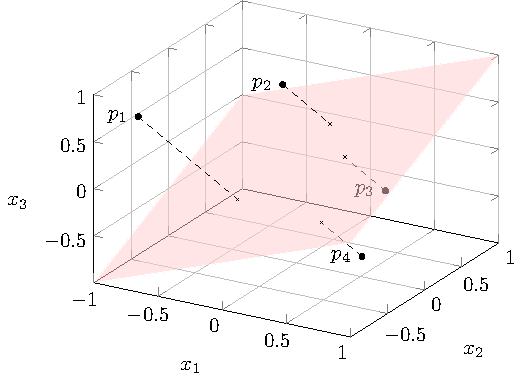
\includegraphics[width=0.8\linewidth]{tikz/random_projection.pdf}
    \caption{Illustration of a random hyperplane (red) partitioning the space}
    \label{fig:rp_3d}
\end{figure}

\begin{definition}[Cosine Similarity]
    The cosine similarity is computed as
    \begin{equation}
        1- \frac{\theta(\bm{p}_1, \bm{p}_2)}{\pi}
    \end{equation}
\end{definition}

Introduced in \cite{charikar2002similarity}, the GRP is defined as follows. Given a message $\bm{x} \in A = \{x \in \mathbb{R}^D : 0 \leq x \leq 1 \}$ and a randomly selected hyperplane defined as $\bm{M}=(a_{ij}) \in \mathbb{R}^{D \times K}$ where $a \sim \mathcal{N}(0, I)$, a \textit{gaussian random projection (GRP)} aims to (\RomanNumeralCaps{1}) reduce the dimensionality from $D$ to $L$ dimensions and (\RomanNumeralCaps{2}) provide a binary encoding by first projecting $\bm{x}$ onto $\bm{M}$ and subsequently applying the sign function to each element of the result, which can be formalized as

\begin{gather}\label{eq:grp_sign}
    h(\bm{x}) = [h(\bm{x}, a_1), \dots, h(\bm{x}, a_k)] \text{ with } h(\bm{x}, a) = sign(\bm{x}^Ta) \\
    \text{with } sign(x) = \Biggl\{ \begin{array}{lc}
        0 & \text{if } x < 0, \\
        1 & \text{if } x \geq 0.
    \end{array}
\end{gather}

An illistration of a random hyperplane that dissects the three-dimensional space and partitions the data space is given in Figure \ref{fig:rp_3d}. The resulting digest $h(x)$ is a binary vector $h(\bm{x}) = \bm{u} \in B = \{0, 1\}^l$ that is used as bucket index for storing $\bm{x}$ in a hash table. For any two messages $\bm{x}_1, \bm{x}_2$, the probability of being hashed to the same bucket increases with a decreasing distance, given as

\begin{equation}\label{eq:rp_proba}
    P[h(\bm{x}_1) = h(\bm{x}_2)] = 1 - \frac{\theta(\bm{x}_1, \bm{x}_2)}{\pi}.
\end{equation}

For a visual proof of the claim in Equation \ref{eq:rp_proba} consider Figure \ref{fig:rp_2d}, where two vectors $p_1$ and $p_2$, regardless of their dimensionality, define a plane and an angle $\theta$ in this plane. Pick a hyperplane $r$ that intersects the plane that is spanned by $p_1$ and $p_2$ in a line (depicted as a red dashed line). Actually, a normal vector $r_0$ is randomly selected and $r$ is the set of points whose dot product with $r_0$ is zero. Since $p_1$ and $p_2$ are on different sides of the hyperplane, their projections given by $\langle p_1, r_0 \rangle$ and  $\langle p_2, r_0 \rangle$ will have different signs. Such a scenario, where two points have different signs, is interpreted as a notion of dissimilarity. Thus, the hyperplane acts as a clustering primitive that partitions the original input set into two disjunct sets.

The opposite scenario is illustrated by a random normal vector $r'_0$ that is normal to the hyperplane $r'$, which is represented by the blue dashed line. Both $\langle p_1, r'_0 \rangle$ and  $\langle p_2, r'_0 \rangle$ will have the same sign. This in turn is interpreted as a notion of similarity, since both points are clustered into the same set. All angles between the intersection line of the random hyperplane and the plane spanned by $p_1$ and $p_2$ are equally likely. Thus, the probability that the hyperplane looks like the red line is $\theta / \pi$ and like the blue line $1 - \theta / \pi$.

Therefore, GRP is a $(R, cR, (1-R/\pi), (1-cR/\pi))$-sensitive family for any $R$ and $cR$. As already explained in Section \ref{subsec:locality-sensitive-hashes}, such a family can be amplified as desired. The AND-construction is refers to the selection of a number of $K$ different random hyperplanes $r_k$. According to the construction in Equation \ref{eq:grp_sign}, all projections $\langle p, r_k \rangle$ for a single point are concatenated into a $K$-bit vector. Likewise, the OR-construction refers to the initialization of a number of $L$ such AND-constructions. The algorithmic procedures for preprocessing and queries from Algorithm \ref{alg:lsh_preprocess} and Algorithm \ref{alg:lsh_query} can be applied withoud change. 

\begin{figure}[t]
    \centering
    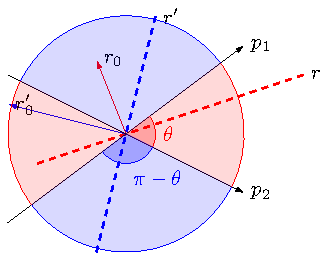
\includegraphics[width=0.6\linewidth]{tikz/random_hyperplane_2d.pdf}
    \caption{Visual Proof of claim in equation \ref{eq:rp_proba}}
    \label{fig:rp_2d}
\end{figure}